\begin{figure}[h] %t-top b-bottom h-here
	\begin{center}
		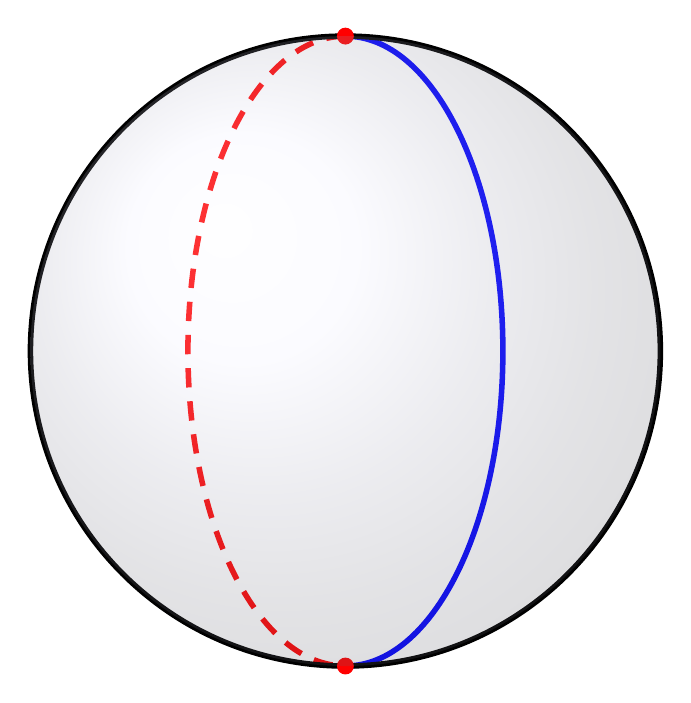
\begin{tikzpicture}%[transform canvas={scale=4.0}]  %%[scale=4] ONLY changes distances, not the canvas
			\draw[blue,line width=2pt] (0,4) arc (90:-90:2cm and 4cm);
			\draw[dash pattern=on 7pt off 5pt,red,line width=2pt] (0,4) arc (90:270:2cm and 4cm);
			\draw[line width=2pt] (0,0) circle (4cm);
			\filldraw[red] (0,4) circle  (0.1); %add fill=, and draw= to have separate colours
			\filldraw[red] (0,-4) circle (0.1);
			\shade[ball color=blue!10!white,opacity=0.20] (0,0) circle (4cm);
		\end{tikzpicture}
	\end{center}
	\caption{красивый сложный, многослойный рисунок}
	\label{fig:circle1}
\end{figure}
